\documentclass[a4paper]{report}

\textwidth 440pt
\textheight 670pt
\oddsidemargin 10pt
\topmargin 0pt
\headsep 0pt
\topskip 5pt
\footskip 30pt


\usepackage{graphicx}

\begin{document}

\title{IIOP.NET architecture documentation}
\author{Dominic Ullmann\\[5mm]
}
\maketitle

\begin{abstract}
This document presents the architecture of IIOP.NET. 
\end{abstract}


\tableofcontents 
\newpage
\listoffigures
\newpage

\chapter{Architecture}

\section{Overview}

\begin{figure}[h]
\begin{center}
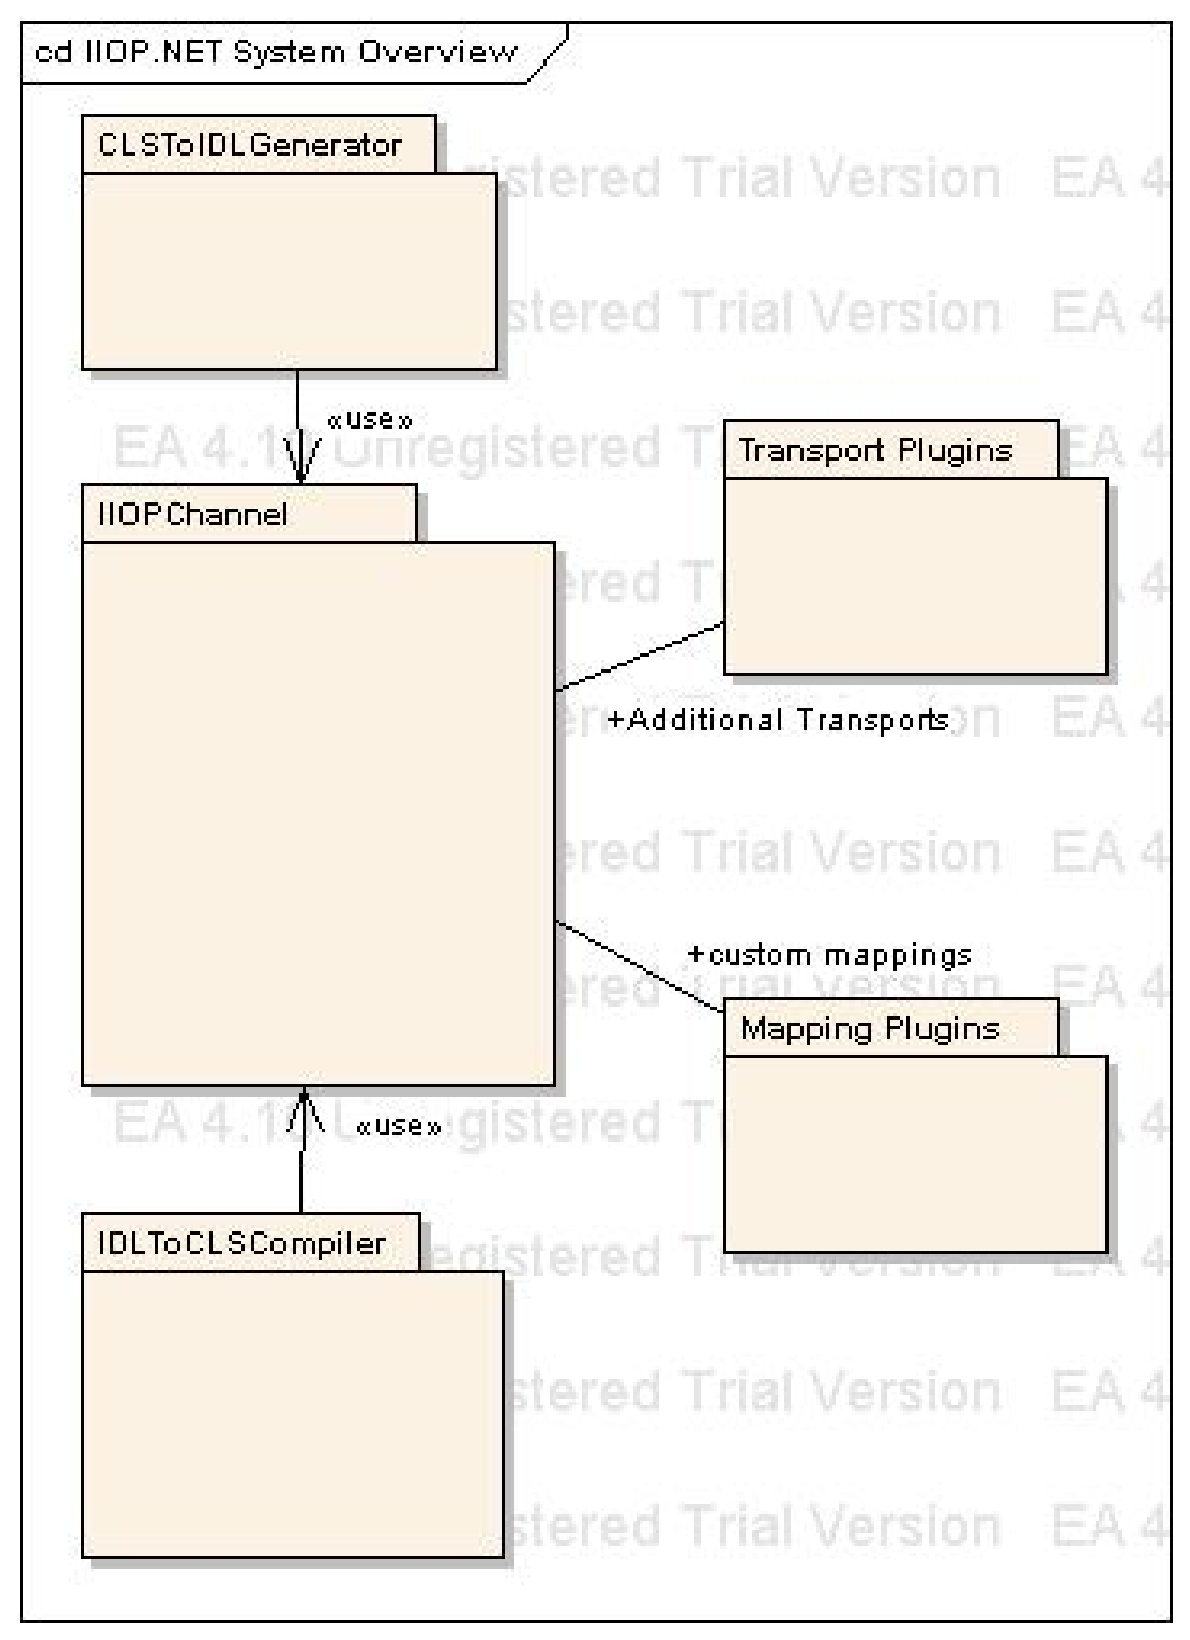
\includegraphics[width=300pt]{DecompOverview.EPS}
\end{center}
\caption{IIOP.NET main parts}
\end{figure}

IIOP.NET consists of the following 3 main parts:
\begin{itemize}
\item IIOPChannel: The .NET remoting channel, allowing to use CORBA/IIOP as remoting protocol.
\item IDLToCLSCompiler: creates .NET assemlies for CORBA IDL.
\item CLSToIDLGenerator: creates CORBA IDL for .NET assemblies.
\end{itemize}

\section{IIOPChannel architecture}
In this chapter the architecture of the IIOPChannel is detailed.

Conceptually, the IIOPChannel consists of the layers detailed in the following figure \ref{IiopChannelLayers}. 
\begin{figure}[h]
\begin{center}
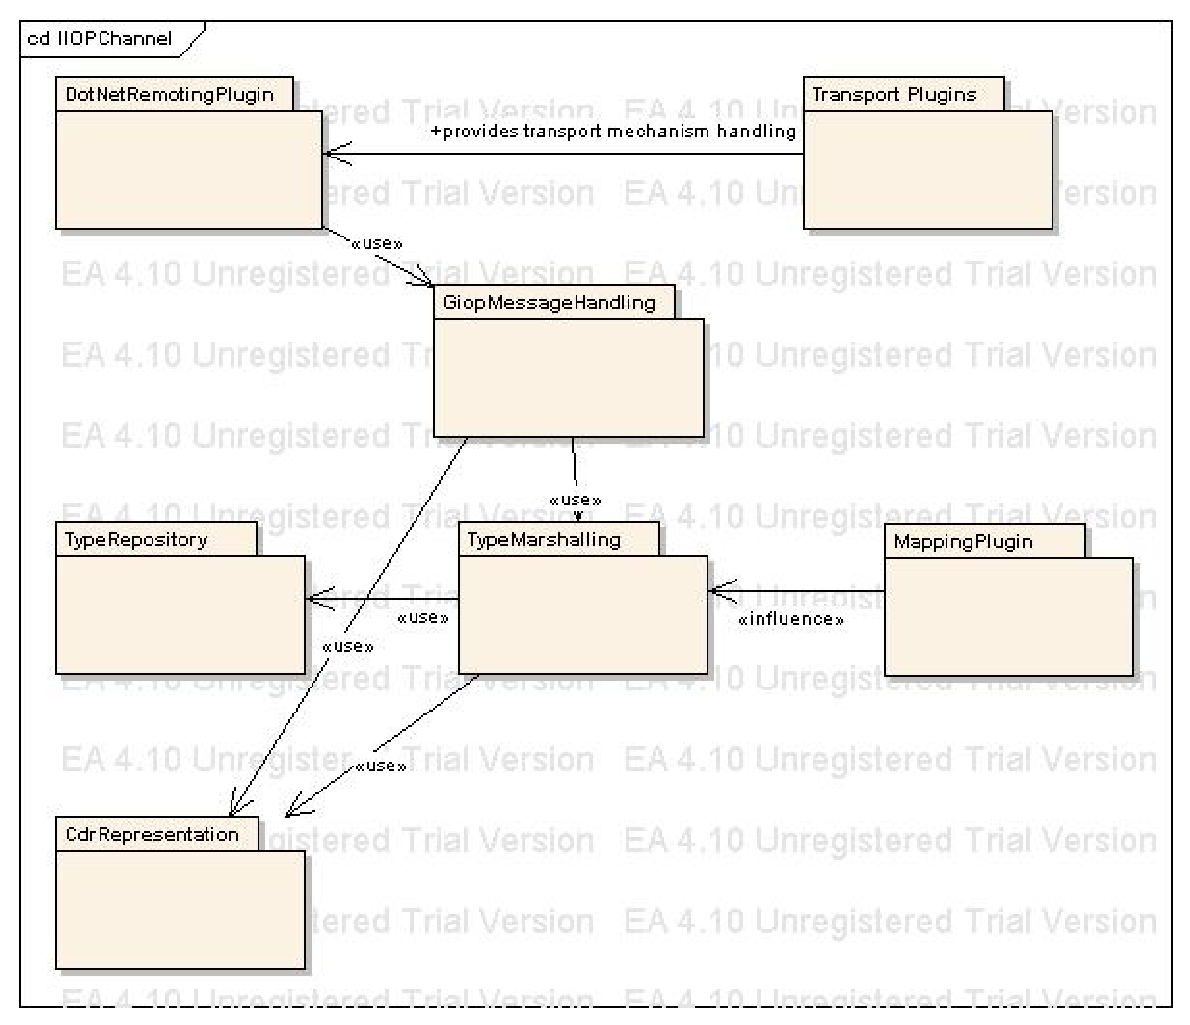
\includegraphics[width=440pt]{IiopChannelLayers.eps}
\end{center}
\caption{\label{IiopChannelLayers} IiopChannel: Layers}
\end{figure}

\subsection{.NET remoting channel implementation layer}

This layer contains the classes, which implement the classes needed for a .NET remoting channel, i.e.
\begin{itemize}
\item The channel classes: IiopChannel, IiopServerChannel, IiopClientChannel
\item The formatter sink classes: IiopClientFormatterSink, IiopServerFormatterSink and the formatter sink providers: IiopClientFormatterSinkProvider, IiopServerFormatterSinkProvider
\item The transport sink classes: IiopClientTransportSink, IiopServerTransportSink and the sink provider for the client side: IiopClientTransportSinkProvider
\end{itemize}
The IiopServerChannel is a channel receiver. It listen for incoming request messages and sends reply messages. The IiopClientChannel
is responsible for sending request messages and receiving the replys.
The IiopChannel wraps those two channels to provide a channel, which is able to send and receive messages.
This wrapper channel allows for example to use callback objects. In this case, the client channel part sends the message containing 
references to the callback object. The sever channel part is then responsible for listening for requests to the callback object.

The formatter classes are responsible for creating the GIOP-messages from .NET remoting messages and for
creating .NET remoting messages from GIOP-messages. The formatter classes use the services provided by the
GIOP message layer to accomplish this task.

The transport classes are responsible for sending and receiving GIOP messages with/from a transport mechanism.
Because some functionality is common to all transport mechanisms, e.g. the reassembling of fragmented GIOP messages,
the transport specific parts are realised with a plugin mechanism. The IIOPChannel already contains
the default plugin for the TCP transport. A transport plugin for SSL is also available.

\subsection{Giop message layer}
This layer is responsible for the handling and the serialization/deserialisation of GIOP Messages. 
The GiopMessage The class GiopMessageHandler gets .NET remoting messages to send from the formatter. It prepares the serialisation and delegates this job
this job to the GiopMessageBodySerialiser. The GiopMessageHandler delegates the deserialisation of GiopMessages to
the GiopMessageBodySerialiser and handle GIOP messages without a counter part in .NET remoting, e.g. ForwardRequest. It
completes the reception job by passing back a .NET remoting message to the formatter.

\subsection{Type marshalling layer}
This layer is responsible for marshalling .NET types as CORBA types and to unmarshal CORBA types to .NET types.

The Marshaller class decides on how to marshal/unmarshal a certain type with the help of the CLStoIDLMapper class and
the SerializerDetermination class. It delegates the serialisation/deserialisation of the different CORBA types 
to the responsible Serialiser.
The MarshallerForType class is a specialisation of the Marshaller, which decides only once
on the mapping for a specific type and than conserves the mapping decision for later reuse.

The Mapping plugin mechanism is able to influence decision of the Marshaller/ClStoIDLMapper to
allow user defined mappings between CORBA and .NET types, e.g. .NET Arrraylist and 
CORBA type for java Arraylist.

The TypeRepository part is responsible to find/load types for Corba type identifiers (repository id's).

%The following figures \ref{TypeMarshallingClasses} and \ref{TypeMarshallingProcedure} illustrates 
%the functionality of this layer.

\subsection{Cdr representation layer}
This layer is responsible for creating/parsing the binary representation of primitive CORBA types.
It contains the CdrStream classes, which can read/write primitive Corba types from/to a stream.
Additionally, there are the CdrEncapsulationStream classes, which are responsible for handling 
Cdr encapsulations.

\newpage
\section{IDL to CLS compiler architecture}
In this chapter the architecture of the IDL To CLS compiler is detailed.

The IDL to CLS compiler is mainly composed of a Console UI, an IDL preprocessor, a Parser and Code generator 
(see figure \ref{IDLcompilerParts}).

\begin{figure}[h]
\begin{center}
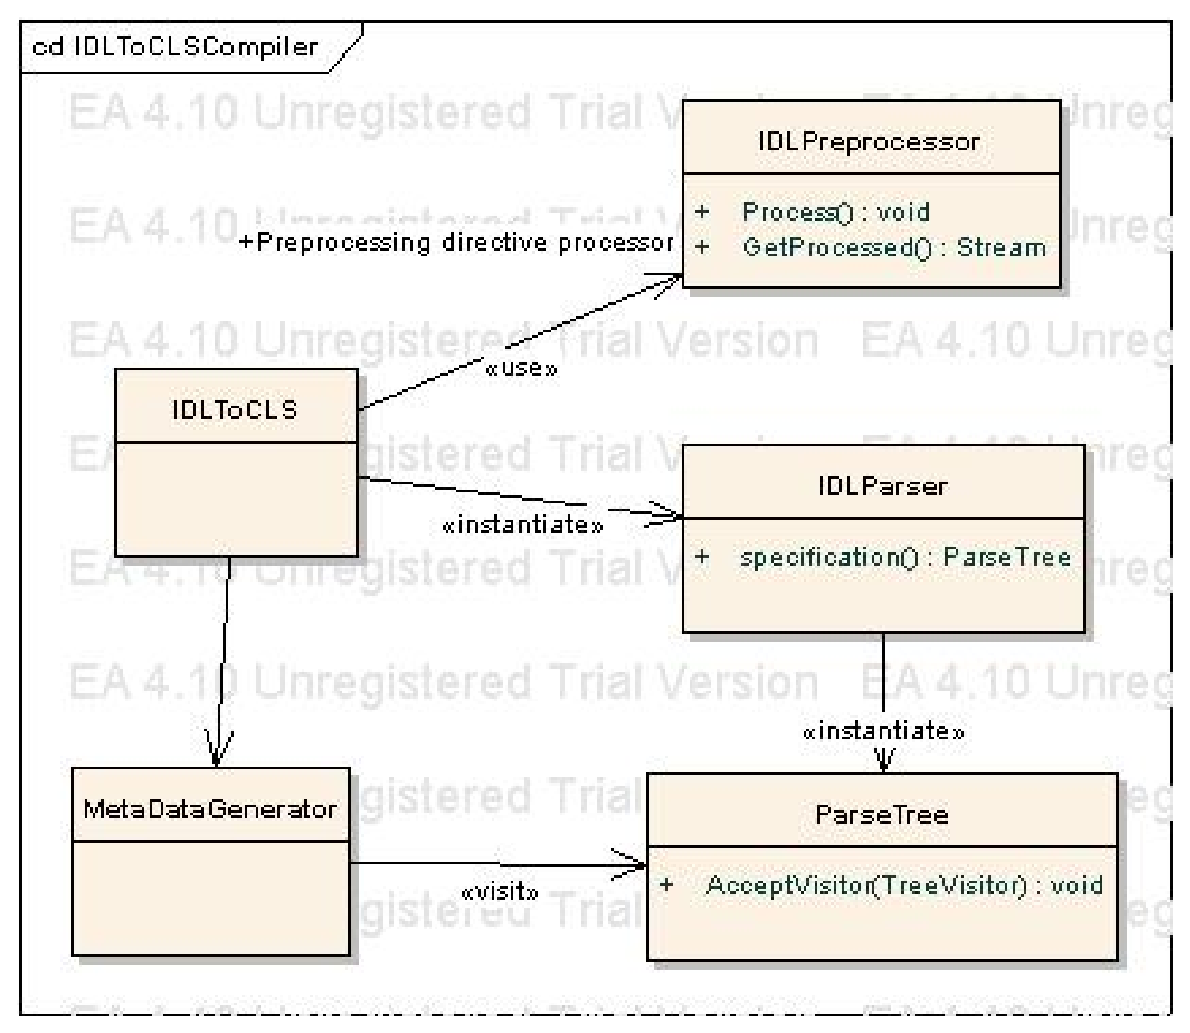
\includegraphics[width=440pt]{IdlCompilerLogical.eps}
\end{center}
\caption{\label{IDLcompilerParts} IDL To CLS compiler main parts}
\end{figure}

The class IDLtoCLS implements the UI part and delegates the compilation work to the preprocessor, parser and code generator.
The IDLPreprocessor class handles the IDL preprocessor directives like include. It passes a preprocessed stream
to the parser for building up an abstract syntax tree (ParseTree). This tree consists of nodes representing the different
constructs in the IDL. This tree supports the visitor pattern. 
The MetadataGenerator is visitor, which generates .NET CLS for the parse tree.
To support building one .NET assembly for multiple independant idl files, this visitor is able
to build code for multiple parse trees one after the other into one assembly.
The process of building a .NET assembly for multiple idl files is shown in figure \ref{IDLCompilerBehaviour}

\begin{figure}[h]
\begin{center}
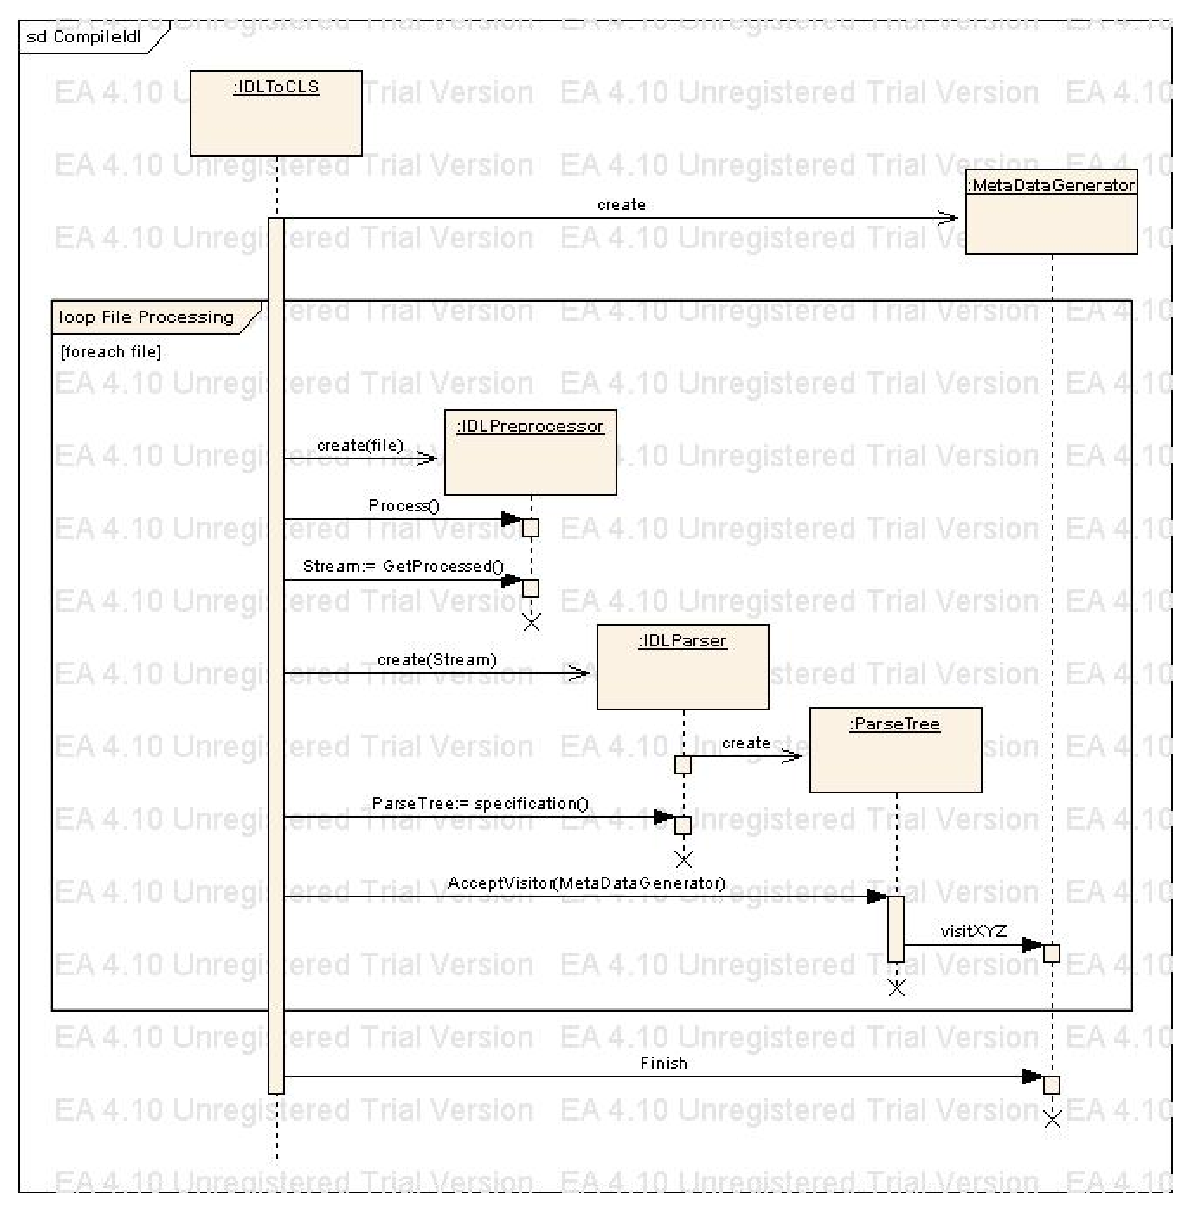
\includegraphics[width=440pt]{IdlCompilerBehaviour.eps}
\end{center}
\caption{\label{IDLCompilerBehaviour} IDL To CLS compiler: processing files}
\end{figure}

\newpage
\section{CLS to IDL generator architecture}
In this chapter the architecture of the CLS to IDL generator is detailed.

\section{extension points}
\subsection{Mapping}
This extension possibility allows to specify custom mappings between .NET and CORBA types.
This is useful, if there are similar types in the .NET and in the peer system, but the
mapping doesn't map them to each other by default, e.g. .NET ArrayList and java ArrayList.

\subsection{Transport protocols}
This extensions allows to send/receive Giop Messages over/with a specific transport protocol, e.g.
TCP or SSL. By default the IIOPChannel contains the Tcp transport protocol plugin. Additionally an
SSL plugin is also part of IIOP.NET.

\end{document}